\documentclass{ximera}
\input{../../preamble.tex}
\addPrintStyle{../..}
\begin{document}
    \author{Zomercursus KU Leuven}
    \xmtitle{Oefeningen goniometrische schrijfwijze van complexe getallen}
    % Start inhoud ximera 


\begin{exercise}
	Schrijf onderstaande getallen in goniometrische vorm $r(\cos\theta+i\sin \theta)$. Zorg er steeds voor dat $\theta$ tussen 0 en $2\pi$ ligt, dus niet $-\frac{\pi}{2}$ invullen maar $\frac{3\pi}{2}$.
	\\
\begin{question} Voor $z=1$ is $r=\answer[onlineshowanswerbutton]{1}$ en $\theta=\answer[onlineshowanswerbutton]{0}$.
\begin{oplossing} 
Omdat $z = 1 = 1 + 0i$ en dus $a = 0$ en $b = 1$, vinden we $|z| = r = 1$. In het complexe vlak zien we dadelijk dat $\theta = 0$.
%Bovendien voldoet $\theta$ aan $\cos \theta = 1$ en $\sin \theta = 0$ zodat $\theta = 0$. 
De goniometrische schrijfwijze van $z$ is dan $z = 1 =  \cos 0 + i\sin 0$.
\begin{image}[0.5\textwidth]
\begin{tikzpicture}[scale = 1, trig format = rad]
	%	grid setup
	
	\def\xmin{-2}
	\def\xmax{2}
	
	\def\ymin{-2}
	\def\ymax{2}				
	
	%	grid
	\draw[step = 1, black, thin, dashed] (\xmin, \ymin) grid (\xmax, \ymax);
	\draw[->] (\xmin, 0) -- (\xmax, 0) node[right]{Re$(z)$};
	\draw[->] (0, \ymin) -- (0, \ymax) node[above]{Im$(z)$};;	
	
	%	vector
	\draw[->, blue, very thick] (0, 0) -- node[below]{$1$}(1, 0);
	
	%	boogje - niet handig nu
	\def\r{0.2}
	%\draw[->, blue] (\r, 0) arc (0:0:\r) node[right]{$0$};
\end{tikzpicture}
\end{image}
\end{oplossing}
\end{question}
    
\begin{question} 
Voor $z=-1$ is $r=\answer[onlineshowanswerbutton]{1}$ en $\theta=\answer[onlineshowanswerbutton]{\pi}$.
\begin{oplossing} 
$z=-1 = -1 + 0i$ en dus $a = -1$ en $b = 0$, waaruit we halen dat $|z| = r = 1$. In het complexe vlak zien we dadelijk dat $\theta = \pi$. 
%Het argument van $z$ moet voldoen aan $\cos \theta = -1$ en $\sin \theta = 0$ zodat $\theta = \pi$. 
De goniometrische schrijfwijze van $z$ is dan $z  = \cos \pi + i\sin \pi$.
\begin{image}[0.5\textwidth]
\begin{tikzpicture}[scale = 1]
	%	grid setup
	
	\def\xmin{-2}
	\def\xmax{2}
	
	\def\ymin{-2}
	\def\ymax{2}				
	
	%	grid
	\draw[step = 1, black, thin, dashed] (\xmin, \ymin) grid (\xmax, \ymax);
	\draw[->] (\xmin, 0) -- (\xmax, 0) node[right]{Re$(z)$};
	\draw[->] (0, \ymin) -- (0, \ymax) node[above]{Im$(z)$};;	
	
	%	vector
	\draw[->, blue, very thick] (0, 0) -- node[below]{$-1$}(-1, 0);
	
	%	boogje - niet handig nu
	\def\r{0.2}
	\draw[->, blue] (\r, 0) arc (0:180:\r) node[midway, above]{$\pi$};
\end{tikzpicture}
\end{image}
Merk op dat de modules positief moet zijn, en met $r=-1$ en $\theta = 0$ is $-(\cos 0 + i\sin0)$ dus \textit{geen} goniometrische schrijfwijze van het getal $-1$.
\end{oplossing}
\end{question}
    
\begin{question} 
Voor $z = i$ is $r = \answer[onlineshowanswerbutton]{1}$ en $\theta = \answer[onlineshowanswerbutton]{\frac{\pi}{2}}$.
\begin{oplossing} 
Omdat $z = i = 0 + i$, en dus $a = 0$, $b = 1$, zodat $|z| = r = 1$. In het complexe vlak zien we dadelijk dat $\theta=\frac{\pi}{2}$.
% en $\theta$ voldoet aan $\cos\theta = 0$ en $\sin \theta = 1$ (of je kan het ook afleiden uit onderstaande schets). 
 De goniometrische schrijfwijze van $z$ is dus $z = \cos \frac{\pi}{2} +i\sin \frac{\pi}{2}$.
\begin{image}[0.5\textwidth]
\begin{tikzpicture}[scale = 1]
	%	grid setup
	
	\def\xmin{-2}
	\def\xmax{2}
	
	\def\ymin{-2}
	\def\ymax{2}				
	
	%	grid
	\draw[step = 1, black, thin, dashed] (\xmin, \ymin) grid (\xmax, \ymax);
	\draw[->] (\xmin, 0) -- (\xmax, 0) node[right]{Re$(z)$};
	\draw[->] (0, \ymin) -- (0, \ymax) node[above]{Im$(z)$};;	
	
	%	vector
	\draw[->, blue, very thick] (0, 0) -- node[left]{$i$}(0, 1);
	
	%	boogje
	\def\r{0.2}
	\draw[->, blue] (\r, 0) arc (0:90:\r) node[midway, right]{$\pi/2$};
\end{tikzpicture}
\end{image}

\end{oplossing}
\end{question}

\begin{question} 
Voor $z = -i$ is $r=\answer[onlineshowanswerbutton]{1}$ en $\theta = \answer[onlineshowanswerbutton]{3\frac{\pi}{2}}$.
\begin{oplossing}
Voor $z = -i$ is $a = 0$ en $b = -1$, dus $|z| = r = 1$. In het complexe vlak zien we dadelijk dat $\theta=\frac{3\pi}{2}$.
% en $\theta$ voldoet aan $\cos \theta = 0$ en $\sin \theta = -1$, dus $\theta = - \frac{\pi}{2} = \frac{3\pi}{2}$. 
 De goniometrische schrijfwijze van $z$ is dus $z  = \cos\left(\frac{3\pi}{2}\right) +i \sin\left(\frac{3\pi}{2}\right)$.
\begin{image}[0.5\textwidth]
\begin{tikzpicture}[scale = 1]
	%	grid setup
	
	\def\xmin{-2}
	\def\xmax{2}
	
	\def\ymin{-2}
	\def\ymax{2}				
	
	%	grid
	\draw[step = 1, black, thin, dashed] (\xmin, \ymin) grid (\xmax, \ymax);
	\draw[->] (\xmin, 0) -- (\xmax, 0) node[right]{Re$(z)$};
	\draw[->] (0, \ymin) -- (0, \ymax) node[above]{Im$(z)$};;	
	
	%	vector
	\draw[->, blue, very thick] (0, 0) -- node[right]{$-i$}(0, -1);
	
	%	boogje
	\def\r{0.2}
	\draw[->, blue] (\r, 0) arc (0:270:\r) node[midway, above]{$\frac{3\pi}{2}$};
\end{tikzpicture}
\end{image}
\end{oplossing}
\end{question}

\begin{question} 
Voor $z = \sqrt{3} + i$ is $r = \answer[onlineshowanswerbutton]{2}$ en $\theta = \answer[onlineshowanswerbutton]{\frac{\pi}{6}}$.
\begin{oplossing} 
Voor $z = \sqrt{3} + i$ geldt $a = \sqrt{3}$ en $b = 1$, dus $|z| = r = \sqrt{a^2 + b^2} = 2$. Het argument van $z$ voldoet aan $\cos \theta = \frac{\sqrt{3}}{2}$ en $\sin \theta = \frac{1}{2}$. Dit zijn de goniometrische getallen van de standaardhoek $\pi/6$. De goniometrische schrijfwijze van $z$ is dus 
$$
z = 2\left(\cos \left(\frac{\pi}{6}\right) + i\sin\left(\frac{\pi}{6}\right)\right) \, .
$$
\begin{image}[0.5\textwidth]
\begin{tikzpicture}[scale = 1.5]
	%	grid setup
	
	\def\xmin{-2.1}
	\def\xmax{2.1}
	
	\def\ymin{-2.1}
	\def\ymax{2.1}				
	
	%	grid
	\draw[step = 1, black, thin, dashed] (\xmin, \ymin) grid (\xmax, \ymax);
	\draw[->] (\xmin, 0) -- (\xmax, 0) node[right]{Re$(z)$};
	\draw[->] (0, \ymin) -- (0, \ymax) node[above]{Im$(z)$};;	
	
	%	vector
	\draw[->, blue, very thick] (0, 0) -- ({sqrt(3)}, 1)node[below]{$\sqrt{3} + i$};
	
	%	boogje
	\def\r{0.5}
	\draw[->, blue] (\r, 0) arc (0:30:\r) node[midway, right]{$\frac{\pi}{6}$};
\end{tikzpicture}
\end{image}
\end{oplossing}
\end{question}
     
\begin{question} 
Voor $z = -\sqrt{3} + i$ is $r = \answer[onlineshowanswerbutton]{2}$ en $\theta = \answer[onlineshowanswerbutton]{\frac{5\pi}{6}}$.
\begin{oplossing} 
Voor $z = -\sqrt{3} + i$ geldt $a = -\sqrt{3}$ en $b = 1$. Dus geldt $|z| = r = 2$. Voor het argument van $z$ geldt dat $\cos \theta = -\frac{\sqrt{3}}{2}$ en $\sin \theta = \frac{1}{2}$. Dan is $\theta =  \frac{5\pi}{6} =\pi -  \frac{\pi}{6}$: dit kan je afleiden uit de goniometrische getallen voor $\pi/6$ en de rekenregels voor supplementaire hoeken te gebruiken.

De goniometrische schrijfwijze van $z$ is dus 
$$
z = 2\left(\cos \left(\frac{5\pi}{6}\right) + i\sin\left(\frac{5\pi}{6}\right)\right) \, .
$$

\begin{image}[0.5\textwidth]
\begin{tikzpicture}[scale = 1.5]
	%	grid setup
	
	\def\xmin{-2.1}
	\def\xmax{2.1}
	
	\def\ymin{-2.1}
	\def\ymax{2.1}				
	
	%	grid
	\draw[step = 1, black, thin, dashed] (\xmin, \ymin) grid (\xmax, \ymax);
	\draw[->] (\xmin, 0) -- (\xmax, 0) node[right]{Re$(z)$};
	\draw[->] (0, \ymin) -- (0, \ymax) node[above]{Im$(z)$};;	
	
	%	vector
	\draw[->, blue, very thick] (0, 0) -- ({-sqrt(3)}, 1)node[below]{$-\sqrt{3} + i$};
	
	%	boogje
	\def\r{0.5}
	\draw[->, blue] (\r, 0) arc (0:150:\r) node[midway, above]{$5\pi/6$};
\end{tikzpicture}
\end{image}
\end{oplossing}
\end{question}
    
\begin{question} 
Voor $z = \cos\frac{\pi}{4}+i\sin\frac{3\pi}{4}$ is $r = \answer[onlineshowanswerbutton]{1}$ en $\theta = \answer[onlineshowanswerbutton]{\frac{\pi}{4}}$.
\begin{oplossing} 
Door supplementaire hoeken te gebruiken vinden we dat 
$$
\sin \left( \frac{3\pi}{4}\right) = \sin \left( \pi-\frac{\pi}{4} \right) = \sin \left(\frac{\pi}{4} \right) \, .
$$
En dus is $z = \cos\frac{\pi}{4}+i\sin\frac{\pi}{4}$: dit is reeds de goniometrische schrijfwijze, met $r = 1$ en $\theta = \frac{\pi}{4}$.
\begin{image}[0.5\textwidth]
\begin{tikzpicture}[scale = 1.8]
	%	grid setup
	
	\def\xmin{-1.5}
	\def\xmax{1.5}
	
	\def\ymin{-1.5}
	\def\ymax{1.5}				
	
	%	grid
	\draw[step = 1, black, thin, dashed] (\xmin, \ymin) grid (\xmax, \ymax);
	\draw[->] (\xmin, 0) -- (\xmax, 0) node[right]{Re$(z)$};
	\draw[->] (0, \ymin) -- (0, \ymax) node[above]{Im$(z)$};;	
	
	%	vector
	\draw[->, blue, very thick] (0, 0) -- ({cos(45)}, {sin(45)}) node[above, fill = white]{$\cos\left(\frac{\pi}{4}\right) + \sin\left(\frac{3\pi}{4}\right) i$};
	
	%	boogje
	\def\r{0.5}
	\draw[->, blue] (\r, 0) arc (0:45:\r) node[midway, right]{$\pi/4$};
\end{tikzpicture}
\end{image}
\end{oplossing}
\end{question}
 
\begin{question} 
Voor $z = \cos\frac{\pi}{3} - i\sin\frac{\pi}{3}$ is $r = \answer[onlineshowanswerbutton]{1}$ en $\theta = \answer[onlineshowanswerbutton]{\frac{5\pi}{3}}$
\begin{oplossing}
Door tegengestelde hoeken te gebruiken vinden we dat $ - \sin\left( \frac{\pi}{3} \right) = \sin \left(-\frac{\pi}{3}\right)$ en $\cos \left(\frac{\pi}{3}\right) = \cos \left(- \frac{\pi}{3} \right)$. Dus $ z = \cos \left(-\frac{\pi}{3}\right) + i\sin \left(-\frac{\pi}{3} \right)$. Als we eisen dat $\theta \in [0, 2\pi]$, dan is de goniometrische vorm van $z$: $z = \cos\frac{5\pi}{3} - i\sin\frac{5\pi}{3}$.

\begin{image}[0.5\textwidth]
\begin{tikzpicture}[scale = 1.5]
	%	grid setup
	
	\def\xmin{-2}
	\def\xmax{2}
	
	\def\ymin{-2}
	\def\ymax{2}				
	
	%	grid
	\draw[step = 1, black, thin, dashed] (\xmin, \ymin) grid (\xmax, \ymax);
	\draw[->] (\xmin, 0) -- (\xmax, 0) node[right]{Re$(z)$};
	\draw[->] (0, \ymin) -- (0, \ymax) node[above]{Im$(z)$};;	
	
	%	vector
	\draw[->, blue, very thick] (0, 0) -- ({cos(-60)}, {sin(-60)}) node[below, fill = white]{$\cos\left(\frac{\pi}{3}\right) - i\sin\left(\frac{\pi}{3}\right)$};
	
	%	boogje
	\def\r{0.5}
	\draw[->, blue] (\r, 0) arc (0:300:\r) node[midway, above]{$5\pi/3$};
\end{tikzpicture}
\end{image}
\end{oplossing}
\end{question}
\end{exercise}

\begin{exercise}
	Bepaal de modulus $|z|$ en het argument $\theta$ van volgende complexe getallen $z$. Geef de hoek $\theta$ in tussen 0 en $2\pi$ radialen.
	
	\begin{question} 
		Als $z=-7i$, dan is $|z|=\answer[onlineshowanswerbutton]{7}$ en $\theta=\answer[onlineshowanswerbutton]{3\pi/2}$.
		\begin{oplossing}
			$z = a + bi = 0 - 7i$, dus is $|z| = \sqrt{a^2 + b^2} = 7$. In het complxe vlak zien we dadelijk dat $\theta = 3 \pi/2$.  Je kan dit ook berekenen:  $\cos\theta=0/7=0$ en $\sin\theta=-7/7=-1$, en dus is $\theta = 3 \pi/2$ (op een veelvoud van $2\pi$ na). 
			
			\begin{image}[0.5\textwidth]
				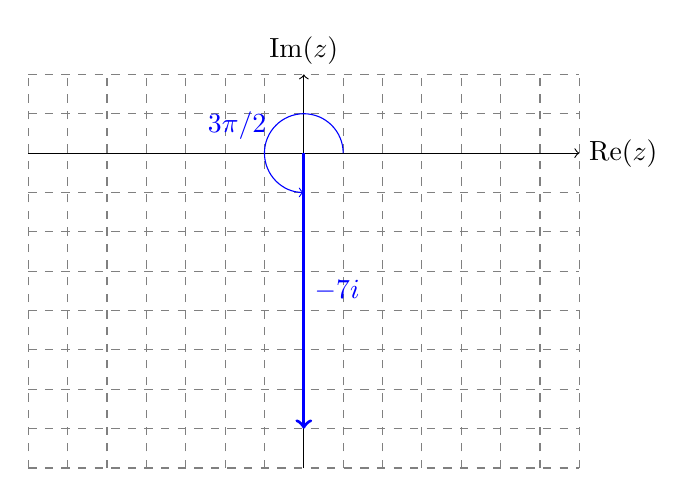
\begin{tikzpicture}[scale = 0.5]
				%	grid setup
				
				\def\xmin{-7}
				\def\xmax{7}
				
				\def\ymin{-8}
				\def\ymax{2}				
				
				%	grid
				\draw[step = 1.0, gray, thin, dashed] (\xmin, \ymin) grid (\xmax, \ymax);
				\draw[->] (\xmin, 0) -- (\xmax, 0) node[right]{Re$(z)$};
				\draw[->] (0, \ymin) -- (0, \ymax) node[above]{Im$(z)$};;	
				
				%	vector
				\draw[->, blue, very thick] (0, 0) -- node[right]{$-7i$}  (0, -7);
				
				%	boogje
				\def\r{1}
				\draw[->, blue] (\r, 0) arc (0:270:\r) node[midway, left]{$3\pi/2$};
				\end{tikzpicture}
			\end{image}
		\end{oplossing}
	\end{question}
	
	
	\begin{question} 
		Als $z=(7i)^{-1}$, dan is $|z|=\answer[onlineshowanswerbutton]{1/7}$ en $\theta=\answer[onlineshowanswerbutton]{3\pi/2}$.
		\begin{hint} Schrijf $z$ eerst in cartesische vorm $a+bi$. \end{hint}
		\begin{oplossing}
			Eerst herschrijven we het complex getal $z$ in cartesische vorm: $z = \frac{1}{7i} = - \frac17 i$ (vermenigvuldig teller en noemer met $i$). 
			\\
			Een tip voor berekeningen met complexe getallen: \textit{delen door $i$ is hetzelfde als vermenigvuldigen met $-i$}.
			
			Omdat $z = a + bi = 0 - \frac17i$ is $|z| = \sqrt{a^2 + b^2} = \frac17$, en $\theta = 3 \pi/2$ (op een veelvoud van $2\pi$ na), zoals we kunnen afleiden uit een schets (de ijk op beide assen is nu 0.1 in plaats van 1):
			
			\begin{image}[0.5\textwidth]
				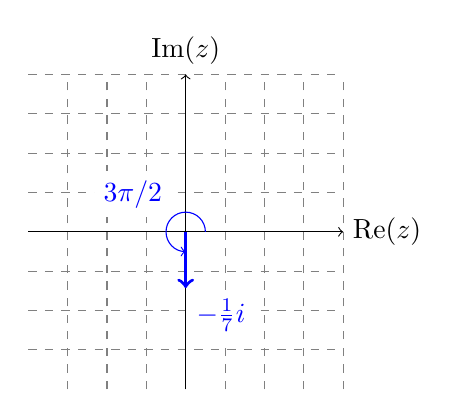
\begin{tikzpicture}[scale = 5]
				%	grid setup
				
				\def\xmin{-0.4}
				\def\xmax{0.4}
				
				\def\ymin{-0.4}
				\def\ymax{0.4}				
				
				%	grid
				\draw[step = 0.1, gray, thin, dashed] (\xmin, \ymin) grid (\xmax, \ymax);
				\draw[->] (\xmin, 0) -- (\xmax, 0) node[right]{Re$(z)$};
				\draw[->] (0, \ymin) -- (0, \ymax) node[above]{Im$(z)$};;	
				
				%	vector
				\draw[->, blue, very thick] (0, 0) -- (0, -1/7) node[below right, fill = white]{$-\frac17i$};
				
				%	boogje
				\def\r{0.05}
				\draw[->, blue] (\r, 0) arc (0:270:\r) node[midway, above left, fill = white]{$3\pi/2$};
				\end{tikzpicture}
			\end{image}
		\end{oplossing}
	\end{question}
	
	
	\begin{question} 
		Als $z = \overline{1+i}$, dan is $|z| = \answer[onlineshowanswerbutton]{\sqrt{2}}$ en $\theta = \answer[onlineshowanswerbutton]{7\pi/4}$.
		\begin{hint} Schrijf $z$ eerst in cartesische vorm $a+bi$. \end{hint}
		\begin{oplossing}
			Eerst herschrijven we het complex getal $z$: $z = \overline{1+i} = 1 - i$.
			
			Omdat $z = a + bi = 1 - i$, is $|z| = \sqrt{a^2 + b^2} = \sqrt{2}$, en $\theta =- \pi / 4$: dit kan je afleiden uit de tekening of bepaal je uit de vergelijkingen 
			%$a = r\cos \theta$ en $b = r\sin\theta$. Deze kan je omvormen naar
			\begin{align*}
			\cos \theta &= \frac{a}{r} = \frac{1}{\sqrt{2}} \\
			\sin \theta &= \frac{b}{r} = -\frac{1}{\sqrt{2}}\\
			\end{align*} 
			We weten dat de cosinus en sinus van de standaardhoek $\pi/4$ beide gelijk zijn aan $\frac{1}{\sqrt{2}}=\frac{\sqrt2}{2}$, en de tegengestelde hoek heeft dezelfde cosinus, maar een tegengestelde sinus. Dus $\theta = - \pi/4$ of $\theta= 7 \pi/4$.
			\begin{image}[0.5\textwidth]
				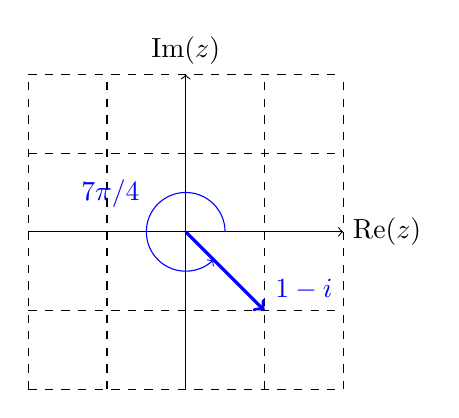
\begin{tikzpicture}[scale = 1]
				%	grid setup
				
				\def\xmin{-2}
				\def\xmax{2}
				
				\def\ymin{-2}
				\def\ymax{2}				
				
				%	grid
				\draw[step = 1, black, thin, dashed] (\xmin, \ymin) grid (\xmax, \ymax);
				\draw[->] (\xmin, 0) -- (\xmax, 0) node[right]{Re$(z)$};
				\draw[->] (0, \ymin) -- (0, \ymax) node[above]{Im$(z)$};;	
				
				%	vector
				\draw[->, blue, very thick] (0, 0) --  (1, -1) node[above right]{$1-i$};
				
				%	boogje
				\def\r{0.5}
				\draw[->, blue] (\r, 0) arc (0:315:\r) node[midway, above left]{$7\pi/4$};
				\end{tikzpicture}
			\end{image}
		\end{oplossing}
	\end{question}
	
	
	\begin{question} 
		Als $z = \dfrac{1-i}{1+i}$, dan is $|z| = \answer[onlineshowanswerbutton]{1}$ en $\theta=\answer[onlineshowanswerbutton]{3\pi/2}$.
		
		\begin{hint} Schrijf $z$ eerst in cartesische vorm $a+bi$. \end{hint}
		\begin{oplossing}
			Eerst herschrijven we het complex getal $z$ naar de vorm $a + bi$:
			$$
			\frac{1-i}{1+i} = \frac{1-i}{1+i} \frac{1-i}{1-i} = \frac{(1-i)^2}{2}= \frac{-2i}{2} = - i 
			$$
			Dan is $|z| = 1$, en in het comlexe vlak zien we dadelijk dat $\theta = 3 \pi/2$.
			\begin{image}[0.5\textwidth]
				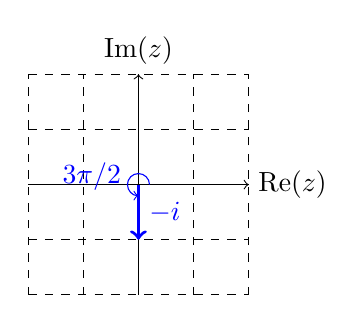
\begin{tikzpicture}[scale = 0.7]
				%	grid setup
				
				\def\xmin{-2}
				\def\xmax{2}
				
				\def\ymin{-2}
				\def\ymax{2}				
				
				%	grid
				\draw[step = 1, black, thin, dashed] (\xmin, \ymin) grid (\xmax, \ymax);
				\draw[->] (\xmin, 0) -- (\xmax, 0) node[right]{Re$(z)$};
				\draw[->] (0, \ymin) -- (0, \ymax) node[above]{Im$(z)$};;	
				
				%	vector
				\draw[->, blue, very thick] (0, 0) -- node[right]{$-i$}  (0, -1);
				
				%	boogje
				\def\r{0.2}
				\draw[->, blue] (\r, 0) arc (0:270:\r) node[midway, left]{$3\pi/2$};
				\end{tikzpicture}
			\end{image}
		\end{oplossing}
	\end{question}    
	
	%%% Volgende oefening in comment: geen standaardhoek, is minder interessant.
	
	
	%\begin{question} 
	%Als $z = \dfrac{1}{1+i}+\dfrac{1+i}{4}$, dan is $|z| = \answer[onlineshowanswerbutton]{\sqrt{10}/4}$ en $\theta=\answer[onlineshowanswerbutton]{-0.32}$.
	%\begin{hint}
	%Om $\theta$ te berekenen, gebruik je best een rekenmachine.
	%\end{hint}
	%\begin{oplossing}
	%Eerst herschrijven we het complex getal $z$ naar de vorm $a + bi$. We doen dit eerst voor de eerste term:
	%$$
	%\frac{1}{1+i} = \frac{1}{1+i} \frac{1-i}{1-i} = \frac{1-i}{2}
	%$$
	%Dan is 
	%$$
	%z = \frac12 - \frac{i}{2} + \frac14  + \frac{i}{4} = \frac34 - \frac14 i \, .
	%$$
	%Dan vinden we dat $|z| = \sqrt{a^2 + b^2} = \sqrt{\frac{10}{16}} = \frac{\sqrt{10}}{4}$. Uit $a = r\cos\theta$ halen we dan dat $\theta = \text{bgcos}\left(\frac{3}{\sqrt{10}}\right)$. Het resultaat kan je nu berekenen met een rekenmachine. 
	%\begin{image}[0.5\textwidth]
	%\begin{tikzpicture}[scale = 1, trig format = rad]
	%	%	grid setup
	%	
	%	\def\xmin{-2}
	%	\def\xmax{2}
	%	
	%	\def\ymin{-2}
	%	\def\ymax{2}				
	%	
	%	%	grid
	%	\draw[step = 1, black, thin, dashed] (\xmin, \ymin) grid (\xmax, \ymax);
	%	\draw[->] (\xmin, 0) -- (\xmax, 0) node[right]{Re$(z)$};
	%	\draw[->] (0, \ymin) -- (0, \ymax) node[above]{Im$(z)$};;	
	%	
	%	%	vector
	%	\draw[->, blue, very thick] (0, 0) -- node[below]{$\frac34 - \frac14 i$}(3/4, -1/4);
	%	
	%	%	boogje
	%	\def\r{0.5}
	%	\draw[->, blue] (\r, 0) arc (0:0.23:\r) node[midway, left]{$0.23$};
	%\end{tikzpicture}
	%\end{image}
	%\end{oplossing}
	%\end{question}    
\end{exercise}



%
%\begin{oefening2}
%	Los volgende vergelijkingen in $z\in \C$ op. Schrijf het resultaat in de vorm $a+bi$.
%	\begin{enumerate}
%		\item $5i \;z+2=3i$
%		\item $(3+i)(z+1)=z$
%		\item $\ds{\frac{7}{z+i}=1-i}$
%		\item $3 z +2 \overline z=10-i$
%		\item $(2+i) \; \overline z =z+4$
%	\end{enumerate}
%	\begin{opl}
%		\begin{enumerate}
%			\item $\frac{3}{5} +\frac{2i}{5}$
%			\item $\frac{-7}{5} +\frac{i}{5}$
%			\item $\frac{7}{2} +\frac{5i}{2}$
%			\item $2-i$
%			\item $3+i$
%		\end{enumerate}
%	\end{opl}
%\end{oefening2}
%
%\begin{oefening2}
%	%An Vanfroyenhoven
%	%\id{2015wis01}
%	
%	Veronderstel dat $x$ en $y$ complexe getallen zijn die voldoen aan het stelsel 
%	\begin{equation*}
%	\begin{cases}
%	(-1-i)x-2y & = 4 \\
%	x+(2-i)y   & = i,
%	\end{cases}
%	\end{equation*}
%	waarbij $i^2=-1$.
%	
%	Bepaal $x+y$.
%	\begin{enumerate}
%		\item [(A)] $x+y=-1+4i$
%		\item [(B)] $x+y=-1+2i$
%		\item [(C)] $x+y=-1$
%		\item [(D)] $x+y=1$
%		\item [(E)] $x+y$ kan oneindig veel waarden aannemen.
%	\end{enumerate}
%	
%	\begin{opl}
%		A 
%	\end{opl}
%	
%	\bron{ijkingstoets juli 2015}
%\end{oefening2}
%
%\begin{oefening2}
%	Bereken
%	\[  \left| \frac{(3+4i)(-1+2i)}{(-1-i)(3-i)}\right|\]
%	\begin{opl}
%		$\ds\frac{5}{2}$
%	\end{opl}
%\end{oefening2}
%
%\newpage
%\begin{oefening2}
%	%\id{2013hds05}
%	%\id{201307beg14**}
%	
%	Als het complex getal $z$ voldoet aan
%	$$
%	z^2 = \frac{(2+i)(-1+2i)}{2(3+4i)}
%	$$
%	dan is de modulus van $z$:
%	\begin{enumerate}
%		\item [(A)]$|z| = \frac{1}{2}$
%		\item [(B)] $|z| = \frac{\sqrt{2}}{2}$
%		\item [(C)]$|z| = \sqrt{2}$
%		\item [(D)]$|z| = - \frac{\sqrt{2}}{2}$
%		\item [(E)]$|z| = \frac{1}{4}$
%	\end{enumerate}
%	
%	
%	\begin{opl}
%		B
%	\end{opl}
%	\bron{ijkingstoets juli 2013}
%	
%\end{oefening2}
%
%\begin{oefening2}
%	%\id{SCvraag1}
%	
%	De getallen $\alpha$ en $\beta$ zijn re\"ele getallen, $i^2=-1$. Als $z_1=1-2i$ een nulpunt is van de complexe
%	veelterm $z^2-(\alpha+i)z+(7+i\beta)$,
%	wat is dan het tweede nulpunt $z_2$?
%	
%	\begin{enumerate}
%		\item [(A)] $z_2=1+2i$
%		\item [(B)] $z_2=1+i$
%		\item [(C)] $z_2=3$
%		\item [(D)] $z_2=1+3i$
%		\item [(E)] $z_2=1-3i$
%	\end{enumerate}
%	
%	
%	\begin{opl}
%		D
%	\end{opl}
%	
%	\bron{ijkingstoets juli 2015}
%\end{oefening2}
%
%%%%%%%%%%%%
%
%%%%%%%%%%%
%
%
%
%
%
%
%
%%%%%%%%%%%%%%
%\begin{oefening2}
%	%\id{2015wis09}
%	
%	Het complexe getal $z$ is de oplossing van de vergelijking $(2+i)(z+i)=z-1$, waarbij $i^2=-1$. Bereken de modulus van $z$.
%	
%	\vspace{4mm}
%	
%	(A) $|z|=1$\hspace{1cm}
%	(B) $|z|=\sqrt 2$ \hspace{1cm}
%	(C) $|z|=2$ \newline
%	(D) $|z|=\sqrt 5$  \hspace{1cm}
%	(E) $|z|=2\sqrt 5$
%	
%	
%	\begin{opl}
%		B
%	\end{opl}
%	%
%	%\cat{vaardigheden}
%	%\class{**}
%	%\info{ijkingstoets september 2015 - 313 deelnemers} 
%	%\juist{62} 
%	%\blanco{23} 
%	%\ul{85/36}
%	\bron{ijkingstoets september 2015}
%\end{oefening2}
%%%%%%%%%
%\newpage
%
%\begin{oefening2}
%	Bereken
%	\begin{enumerate} \item  $(-1-i)^{20}$
%		\item $(1+i)^{21}$
%		\item $(-\sqrt{3}+i)^5$
%	\end{enumerate}
%	\begin{opl}\mbox{}
%		\begin{enumerate}
%			\item $-1024$
%			\item $-1024-1024i$
%			\item $16\sqrt{3}+16i$
%		\end{enumerate}
%	\end{opl}
%\end{oefening2}
%
%\begin{oefening2}
%	Los op in $\C$ en geef de ontbinding in factoren.
%	\begin{enumerate}
%		\item $-x^2+x-2=0\qquad$
%		\item  $ 2x^2-10x+13=0\qquad$
%		\item  $ 3x^2-5x+7=0\qquad$
%	\end{enumerate}
%	
%	\begin{opl}
%		\begin{enumerate}
%			\item $x_{1,2}=\frac{1\pm i \sqrt{7} }{2}$, de ontbinding is
%			$-x^2+x-2=-1(x-\frac{1+ i \sqrt{7}}{2})(x-\frac{1- i
%				\sqrt{7}}{2})$
%			\item $x_{1,2}=\frac{5\pm i}{2}$, de ontbinding is
%			$2x^2-10x+13=2(x-\frac{5+ i}{2})(x-\frac{5-i}{2})$
%			\item $x_{1,2}=\frac{5\pm i \sqrt{59} }{6}$, de ontbinding is
%			$3x^2-5x+7=3(x-\frac{5+ i \sqrt{59} }{6})(x-\frac{5- i \sqrt{59}
%			}{6})$
%		\end{enumerate}
%	\end{opl}
%\end{oefening2}
%
%\begin{oefening2}
%	Zoek een vierkantsvergelijking met re\"ele co\"effici\"enten
%	waarvan $3+2i$  een wortel is.
%	\begin{opl}
%		$x^2-6x+13=0$
%	\end{opl}
%\end{oefening2}
%
%\begin{oefening2}
%	Zoek alle complexe wortels van volgende vergelijking
%	$(x^2+5)(x^3+x-2)=0.$
%	\begin{opl}
%		$\pm\sqrt{5}\;i, 1,\ds \frac{-1\pm\sqrt{7}\;i}{2}$
%	\end{opl}
%\end{oefening2}
%
%
%\begin{oefening2}
%	Los de binomiaalvergelijking $z^3=1+i$ op. Stel de
%	oplossingen voor in het complex vlak.
%\end{oefening2}
%
%\begin{oefening2}
%	Beschouw een $z\in\C$ met $|z|=1$.
%	\begin{enumerate}
%		\item Toon aan dat $\left(\ds\frac{1+z}{|1+z|}\right)^2=z.$
%		\item Kan je dat resultaat ook meetkundig verklaren? Teken daartoe
%		$z$ (ergens op de eenheidscirkel), waar ligt dan $1+z$ en $\ds
%		\ds\frac{1+z}{|1+z|}\;\dots$?
%	\end{enumerate}
%\end{oefening2}
%
%




\end{document}
